\chapter{Rozwiązania chmurowe}

\section{Microsoft Azure}

Aby zapewnić wysoki poziom bezpieczeństwa oraz dostępności systemu zdecydowano się na skorzystanie z~chmury Micrsoft Azure.
Wykorzystany został serwer wirtualny, na którym zainstalowano system Ubuntu 16.04 LTS. Dostęp do serwera możliwy jest wyłącznie po protokole SSH.

\paragraph{Parametry maszyny wirtualnej 'Anton'}
\begin{itemize}
    \item \textbf{Klasa}: B2MS
    \item \textbf{Lokalizacja}: Zachodnia Europa
    \item \textbf{Moc obliczeniowa}: 2 vCPU
    \item \textbf{Pamięć RAM}: 8 GB
    \item \textbf{Dysk SSD}: 16 GB
    \item \textbf{Ilość dysków danych}: 4
    \item \textbf{Ilość operacji wejścia/wyjścia na sekundę}: 4800
    \item \textbf{Koszt}: 60,98 € miesięcznie
\end{itemize}

Po skonfigurowaniu środowisk deweloperskich zarówno dla części obsługującej aplikacje mobilne oraz części odpowiedzialnej za przetwarzanie obrazu, wybrany katalog podłączono do repozytorium kodu korzystającego z systemu kontroli wersji "git", które znajduje się w~serwisie GitHub.com.
W ten sposób bieżące zmiany były dokonywane na komputerach deweloperów, którzy za pomocą repozytorium publikowali nowe wersje aplikacji serwerowej w~chmurze.

\section{Firebase}

W~celu usprawnienia działania aplikacji klienckich skorzystano także z~usług platformy Firebase. Platforma Firebase jest częścią chmury Google Cloud i~oferuje między innymi:

\begin{itemize}
    \item \textbf{Firebase Auth} - usługę bezpiecznej autoryzacji użytkowników ,
    \item \textbf{Firebase Storage} - usługę wygodnego przechowywania plików,
    \item \textbf{Firebase Realtime Database} - usługę bazy danych aktualizowanej w czasie rzeczywistym.
\end{itemize}

Usługi autoryzacji użytkowników zostały wykorzystane nie tylko w aplikacjach klienckich, ale i~także na serwerze do autoryzacji tokenów z~nadchodzących żądań klientów. Usługa przechowywania plików została wykorzystywana do przesyłania fragmentów nagrań na których wykryto niebezpieczeństwo. Usługa bazy danych została wykorzystana do prezentowania w~czasie rzeczywistym wartości czujników w~aplikacjach klienckich.


\section{Aplikacja serwerowa}

Serwer, obsługujący aplikacje mobilne, wykonano we frameworku języka Python - Django, z~wykorzystaniem modułu Django-Rest-Framework. Umożliwił on tworzenie endpointów, które, zgodnie z~rozdziałem nt. komunikacji, które mogły odbierać zapytania POST.
Obsługę zapytań można podzielić, ze względu na zaplanowane źródło zapytania: aplikacja użytkownika lub urządzenie Raspberry.
W~pierwszej kolejności przedstawione zostaną wiadomości wymieniane na linii Raspberry - Serwer.
\paragraph{a) Rejestracja Raspberry Pi:}
\begin{verbatim}
Adres: /backend/v1/devices/add
Zawartość:
{
	'serial': <serial-urządzenia>, 
	'name': <nazwa-urządzenia>, 
	'token': 'jwt.token.from.client'
}
\end{verbatim}
Działanie: Raspberry, o~podanym numerze seryjnym i~nazwie, zostaje dodane do bazy danych urządzeń.

\paragraph{b) Wykrycie ruchu:}
\begin{verbatim}
Adres: /backend/v1/PIRnotification
Zawartość: 
{
	'serial': <serial-urządzenia>, 
	'message': <wiadomość>, 
	'token': 'jwt.token.from.client'
}
\end{verbatim}
Działanie: Po odebraniu informacji o~wykryciu ruchu, następuje pobranie klatki ze strumienia obrazu nadawanego przez Raspberry o~wskazanym numerze seryjnym. Jeżeli na pobranej klatce wykryto człowieka, uruchamiana jest funkcja nagrywająca 30 sekundowy fragment wideo, który zostaje zapisany w~bazie danych Firebase Storage. Użytkownik zostaje poinformowany o~zajściu zdarzenia z~informacją zawartą w polu 'message'. Notyfikacja zostanie wysłana jeżeli wykrycie ruchu zostało spowodowane przez człowieka. W~każdym innym przypadku zostanie zignorowana.

\paragraph{c) Wykrycie zmian na czujniku:}
\begin{verbatim}
Adres: /backend/v1/notification
Zawartość: 
{
	'serial': <serial-urządzenia>, 
	'sensorType': <typ-czujnika>, 
	'value': <wartość>, 
	'token': `jwt.token.from.client`
}
\end{verbatim}
Działanie: Informuje serwer o~wykryciu zagrożenia na jednym z~czujników. Serwer następnie wyszukuje wszystkich klientów, którzy posiadają urządzenie o~numerze seryjnym, który wykrył niebezpieczne wskazania na czujniku i~wysyła do nich powiadomienie za pomocą push notyfikacji. \newline
Następne zapytania dotyczą poleceń wysyłanych z~aplikacji użytkownika.
\paragraph{d) Pobranie urządzeń użytkownika:}
\begin{verbatim}
Adres: /backend/v1/get
Zawartość: 
{
	'owner':<użytkownik>, 
	'token': 'jwt.token.from.client'
}
\end{verbatim}
Działanie: Zwraca listę urządzeń użytkownika.
\paragraph{e) Zmiana nazwy urządzenia:}
\begin{verbatim}
Adres: /backend/v1/devices/changeRaspName
Zawartość:
{
	'serial': <serial-urządzenia>, 
	'name': <nowa-nazwa>, 
	'token': 'jwt.token.from.client'
}
\end{verbatim}
Działanie: Zmienia nazwę urządzenia, wyświetlaną w~aplikacji użytkownika. Przyjęto, że nazwa ta powinna oznaczać miejsce, w~którym znajduje się urządzenie.
\paragraph{f) Uzbrojenie/rozbrojenie urządzenia:}
\begin{verbatim}
Adres: /backend/v1/devices/changeIsArmed

Zawartość: 
{
	'serial': <serial-urządzenia>, 
	'armed': <nowy-stan>, 
	'token': 'jwt.token.from.client'
}
\end{verbatim}
Działanie: Ustala czy nowe powiadomienia związane z~urządzeniem dalej będą wysyłane do aplikacji.
\paragraph{g) Pobranie listy notyfikacji:}
\begin{verbatim}
Adres: /backend/v1/devices/getNotifications
Zawartość: 
{
	'serial': <serial-urządzenia>,  
	'token': 'jwt.token.from.client'
}
\end{verbatim}
Działanie: Pobiera listę notyfikacji (historię zdarzeń) powiązanych z~urządzeniem o~podanym numerze seryjnym.
\paragraph{h) Powiązanie aplikacji z kontem użytkownika:}
\begin{verbatim}
Adres: /backend/v1/devices/fcmTokenUpdate
Zawartość: 
{
	'email': <użytkownik>, 
	'fcmToken': <token-z-firebase>, 
	'deviceId' : <id_aplikacji>
}
\end{verbatim}
Działanie: Powiązuje aplikację mobilną jak i~sesję aplikacji przeglądarkowej o~podanym tokenie z~kontem użytkownika. Dzięki temu, notyfikacje trafiają na wszystkie urządzenia użytkownika.
\newline
\newline
Wybrane rozwiązanie pozwala na łatwą lokalizację ewentualnego błędu w działaniu systemu oraz szybką jego naprawę. Ponadto prosta logika oraz łatwe i~krótkie funkcje obsługujące zapytania sprawiają, że dalszy rozwój tej części systemu będzie możliwy bardzo niskim nakładem sił. 

\section{Baza danych}
System bazuje na dwóch oddzielnych bazach danych. Pierwsza z~nich zawiera wyłącznie dane z~czujników pomiarowych, druga całą resztę. Dane z~czujników pomiarowych aktualizowane są bardzo często i~wymagają natychmiastowego asynchronicznego przesłania tej informacji do klientów. To było powodem przeniesienia tej tabeli do zewnętrznego systemu, który posiada już takie rozwiązania. Zdecydowano się na usługę Firebase, ponieważ oferuje właśnie te dwie bardzo ważne funkcjonalności.  Dane niewymagające częstych zmian znajdują się w bazie danych Django.

\paragraph{Baza danych Firebase}
Baza danych firebase opiera się na strukturze JSON czyli na elementach klucz-wartość. Nie istnieje tu podział na kolumny i~wiersze jak w przypadku standardowej relacyjnej bazy danych. Dane z~czujników zapisywane są wewnątrz elementu nadrzędnego w~strukturze reprezentującego numer seryjny urządzenia Raspberry Pi, z~którego dane pochodzą (Rys. \ref{json}). Wewnątrz kluczy z~nazwami typów czujników znajdują się wartości zmierzone na nich wcześniej i~przechowywane są w polu 'value'. Za aktualizację tej struktury odpowiada oprogramowanie uruchomione na Raspberry.
\begin{figure}[H]
   \centering
   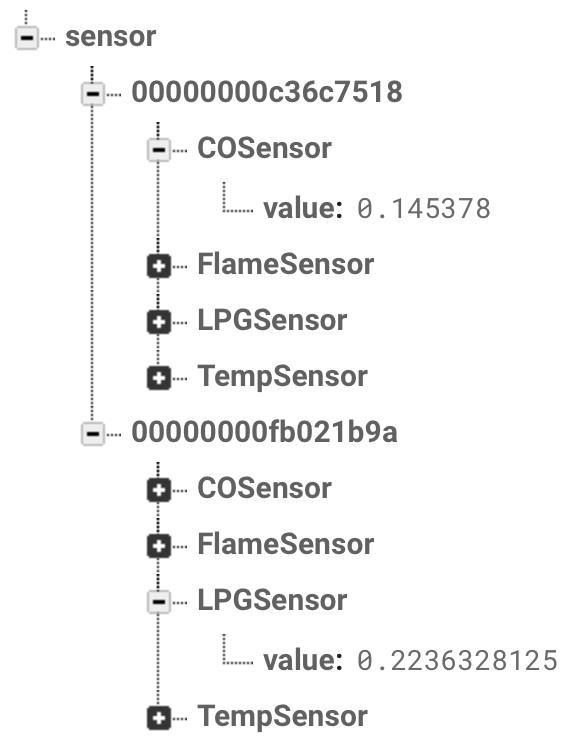
\includegraphics[width=4cm]{firebasejson.png} 
   \caption{Struktura bazy danych Firebase [źródło własne]}
   \label{json}
\end{figure}

\paragraph{Baza danych Django} została zaimplementowana w SQlite3 i~poza specyficznymi dla bibliteki tabelami zawiera:
\begin{itemize}
	\item \textbf{backend\_fcmtokens} przechowuje trzy wartości: aktualny token, id urządzenia oraz nazwę konta (e-mail). Na podstawie tokenu zachodzi autoryzacja urządzeń mobilnych.
	\item \textbf{backend\_notification} zawiera notyfikacje wraz z~ich typem, informacją z~którego urządzenia pochodzą, datą, wiadomością przesłaną razem z notyfikacją oraz adresem url wideo (jeśli takie zostało dołączone do wiadomości)
	\item \textbf{backend\_rasps} zawiera informację nt. urządzenia: jego numer seryjny, nazwę, konto do którego jest przypisane, stan (czy urządzenie przesyła notyfikacje)
	\item \textbf{users\_user} -~jest to tabela zawierająca dane użytkowników logujących się w~aplikacji internetowej (w~szczególności ich login i hasło, identyczny z~tymi przechowywanymi w~usłudze Firebase Auth)
\end{itemize}
